\documentclass[10pt, conference, compsocconf]{IEEEtran}

% packages
\usepackage{algorithm}
\usepackage{algorithmic}
\usepackage{amsfonts} % for R symbol (the set of real numbers)
\usepackage{color}
\usepackage[pdftex]{graphicx}
\usepackage{graphicx}
\usepackage[bookmarks=false]{hyperref}
\hypersetup{colorlinks=true,linkcolor=black,citecolor=black,filecolor=black,urlcolor=blue}
\usepackage{mathtools}
\usepackage{multirow}
\usepackage{stmaryrd} % for llbracket and rrbracket
\usepackage{subcaption}
\DeclarePairedDelimiter{\ceil}{\lceil}{\rceil}
\DeclarePairedDelimiter{\floor}{\lfloor}{\rfloor}

% new commands
\newcommand{\todo}[1]{\marginpar{\parbox{18mm}{\flushleft\tiny\color{red}\textbf{TODO}:
      #1}}}
\newcommand{\comment}[1]{\marginpar{\parbox{18mm}{\flushleft\tiny\color{blue}\textbf{Comment}:
      #1}}}

\newcommand{\note}[1]{
  \color{blue}\emph{[Note: #1]}
  \color{black}
}

\begin{document}

\title{Predicting computational reproducibility of scientific pipelines using collaborative filtering}

\author{Soudabeh Barghi, Lalet Scaria, Tristan Glatard\\
  Department of Computer Science and Software Engineering\\ Concordia University, Montreal, Quebec, Canada\\
  {first.last}@concordia.ca\\
  $^*$ These authors have contributed equally
}

\maketitle

\begin{abstract}
\end{abstract}


\section{Introduction}

Computational reproducibility, the property through which
computational results can be recomputed over time and
space~\cite{stodden}, has become a critical component of scientific
methodology with the rise of the reproducibility crisis in several
domains~\cite{xxx}. Among the factors hampering computational
reproducibility, infrastructural characteristics such as the operating
system play an important role. In neurosciences, our primary field of
interest, several studies have shown the effect of the operating
system on computational results. However, conducting such
reproducibility studies at scale is cumbersome due to the execution
time of data analysis pipelines, which easily exceeds a few hours.

In this paper we investigate approximate methods to predict the
reproducibility of a computational analysis from the first files that
it produces. Our main intuition is that reproducibility errors are
caused by a reduced number of factors that originate in the analysis
pipeline and input data. 

% Computational reproducibility is an issue, for instance among
% different operating systems (refer to Glatard FINF 2015,
% Gronenschild 2012).

% Scientific data analysis pipeline executions are long (give examples
% from neuroimaging).

% Refer to Germain et al 2008.

% Define subjects, pipelines.

% Problem: predict the reproducibility of pipeline files from other
% subjects and the first files produced by a pipeline. Restrict the
% study to binary classification.




\section{Method}

what is specific to our problem compared to regular collaborative filtering:
%+ subjects are equivalent to users. Not all subjects have the same input data. Anatomical variability, acquisition variability (e.g., 1 subject may have multiple T1s).
%+ files are produced in a specific order (movies aren't),
% which add constraints on the training set (cannot sample late files and not early ones).
%+ utility matrix is not sparse: we can potentially populate it completely. Which means that we can decide precisely which samples we need (active sampling). Therefore we can take the first row and first column to avoid cold start issues.

\subsection{Collaborative filtering using ALS}

We consider the collaborative filtering method as implemented in Spark's MLlb.
% Summarize Koren, Bell and Volinsky: https://dl.acm.org/citation.cfm?id=1608614

% Explain that you have binary classes (rounding)

% Biases


\subsection{Sampling the training set}

We investigated the following sampling techniques for the training set. 
In each method, we included the first row of the matrix (first 
generated file of each subject) and a random column (all files of a 
random subject) to avoid cold start issues. \todo{Check why the first line is not in random unreal}

% Explain all sampling techniques (maybe rename 4, 5, and 6)
% 1. random unreal (baseline)
\paragraph{Random Unreal}
The training set is sampled randomly with no restriction, that is,
regardless of the file generation time. This method will be used as a
baseline for comparison with other methods, although it is not
realistic. Figure~\ref{fig:Random-Unreal-Sample-Training-set} represents 
a training set sampled using this method.


% 2. columns
\paragraph{Complete Columns}
The training set is sampled by randomly selecting complete columns in
the matrix, that is, complete subject executions. The last selected
column might be incomplete to meet the exact training ratio. This 
method is realistic: it corresponds to a situation where the 
collaborative filtering method will predict the reproducibility in the 
remaining subjects from the subjects in the training set. 
Figure~\ref{fig:Columns-Sample-Training-set} represents a training set 
sampled using this method.


% 3. rows
\paragraph{Complete Rows} The training set is sampled by selecting complete 
rows in the matrix, that is, the first files produced by
every execution. The last selected row might be incomplete to meet the
exact training ratio. This method is realistic: it corresponds to a 
situation where the processing of all the subjects is launched and 
interrupted before the execution is complete. The collaborative 
filtering method will then predict the reproducibility of the remaining 
files. Figure~\ref{fig:Rows-Sample-Training-set} represents a training 
set sampled using this method.
\begin{figure}[h!]
	\centering
	\begin{subfigure}[b]{0.4\linewidth}
		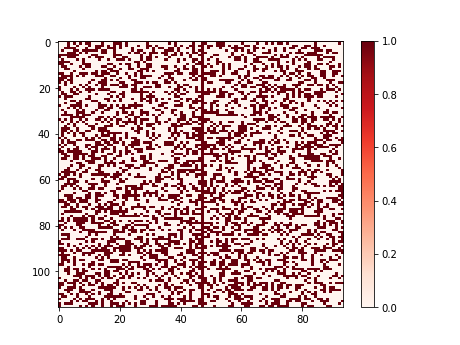
\includegraphics[width=\columnwidth]{figures/5vs7_random-unreal_04_training}
  		\caption{Random Unreal method}
  		\label{fig:Random-Unreal-Sample-Training-set}
	\end{subfigure}
	\begin{subfigure}[b]{0.4\linewidth}
  		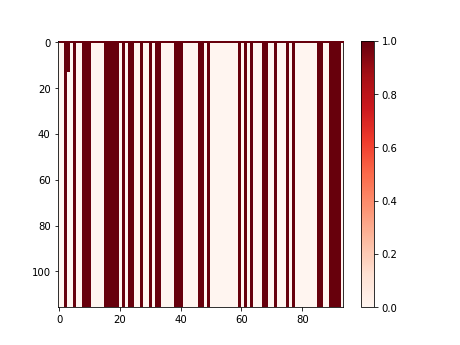
\includegraphics[width=\columnwidth]{figures/5vs7_columns_04_training}
  		\caption{Complete Columns method}
  		\label{fig:Columns-Sample-Training-set}
	\end{subfigure}
	\begin{subfigure}[b]{0.4\linewidth}
  		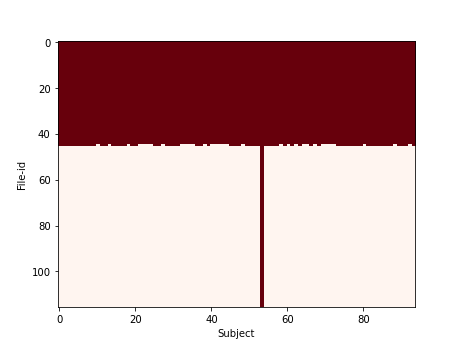
\includegraphics[width=\columnwidth]{figures/5vs7_rows_04_training}
  		\caption{Complete Rows method}
  		\label{fig:Rows-Sample-Training-set}
	\end{subfigure}
	\begin{subfigure}[b]{0.4\linewidth}
 		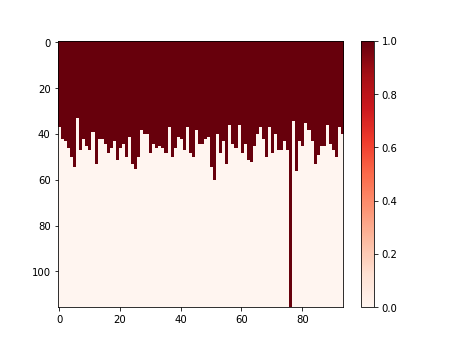
\includegraphics[width=\columnwidth]{figures/5vs7_random-real_04_training}
		\caption{Random Subjects method}
  		\label{fig:Uniform-S-Sample-Training-set}
	\end{subfigure}
	\begin{subfigure}[b]{0.4\linewidth}
  		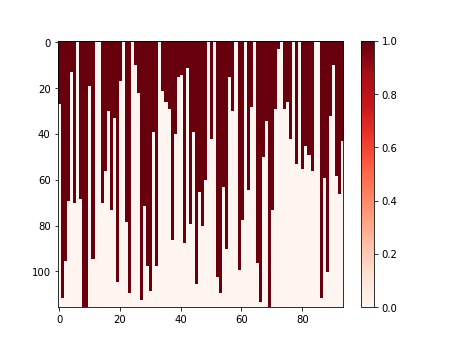
\includegraphics[width=\columnwidth]{figures/5vs7_diagonal_04_training}
  		\caption{(Uniform) method }
  		\label{fig:Diagonal-Sample-Training-set}
	\end{subfigure}
	\begin{subfigure}[b]{0.4\linewidth}
  		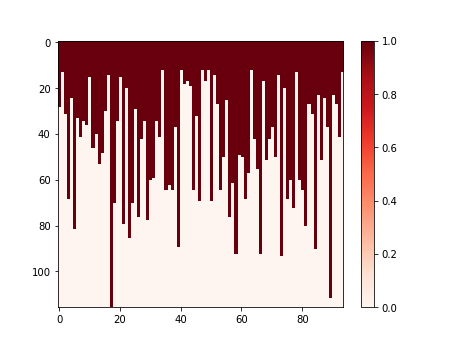
\includegraphics[width=\columnwidth]{figures/5vs7_random-triangular-largest_04_training}
  		\caption{(Triangular-L) method}
  		\label{fig:triangular-L-Sample-Training-set}
	\end{subfigure}
	\begin{subfigure}[b]{0.4\linewidth}
  		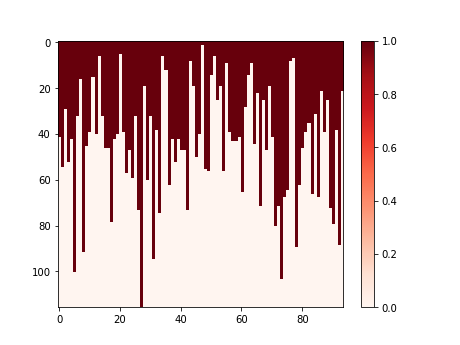
\includegraphics[width=\columnwidth]{figures/5vs7_random-triangular-smallest_04_training}
  		\caption{(Triangular-S) method}
  		\label{fig:triangular-S-Sample-Training-set}
	\end{subfigure}
	\caption{Sample training set for different methods with a training ratio of 0.4.}		
\end{figure}

\paragraph{Random Subjects -- RS} This method builds the 
training set by selecting the files from random subjects 
until the training ratio is reached. The file selected in a 
subject is the file with the lowest index in this subject that has not 
been already selected in the training set. This method is realistic as 
files are sampled according to their production timestamps. 
Figure~\ref{fig:Uniform-S-Sample-Training-set} represents a training 
set sampled using this method.

\paragraph{Random File Numbers (Uniform) -- RFNU}

The number of files selected for every subject is randomly selected in 
a uniform distribution with parameters \textit{\textbf{a}} and 
\textit{\textbf{b}} where \textit{\textbf{b}} is set to the total 
number of files $N_{f}$ and \textit{\textbf{a}} is set such that the 
distribution average equals to $\alpha N_{f}$ where $\alpha$ is the training ratio,  that is, 
$\textit{\textbf{a}}=(2\alpha-1)N_{f}$. \todo{Explain what you do when alpha is lower than 0.5}

This method is realistic as files are sampled according to their production timestamps.
Due to sampling issues, it is possible that the actual training ratio obtained with this method
does not match the target one. We check that the difference between the target and real training ratios
was lower than 0.01. 

\paragraph{Random File Numbers (Triangular) -- RFNT}
The number of files selected in every subject is randomly selected in a triangular distribution
with parameters a, b and c where a, b and c are set as follows: \ldots{}
This distribution aims at sampling files produced towards the end of the execution.
Two approches are tried to apply this method:
\begin{enumerate}
\item Largest-a (RFNT-L):  In this approach there is a concern to eliminate the possibility of having less \todo{Reformulate, this is unclear.}
than the two first generated files of any subjects in the sampled training set. 
The possibility of missing some subjects in training set can happen to some of them due to 
random selection of subjects or even meeting the determined training ratio before 
having the chance of being selected.

\item Smallest-a (RNFT-S): In this approach of utilizing triangular distribution,despite of Largest-a approch, there is a possibility 
that some subjects be reperesented in the training set just by their first generated file and no more files. \todo{Reformulate, this is unclear.}

\end{enumerate}

\section{Dataset}

We collected data to evaluate the computational reproducibility of analysis
pipelines of the Human Connectome Project~\cite{general-hcp}. We
processed a set S of 94 subjects randomly selected in the S500 HCP
release~\todo{URL} in three execution conditions with different
versions of the CentOS operating system (5.?, 6.? and 7.?), using the
PreFreesurfer, Freesurfer, PostFreesurfer and fMRIVolume pipelines
described in~\cite{hcp-pipelines} and available at \todo{URL}. For
each pipeline, we identified the set F of files produced for all
subjects in all conditions. For each condition pair and each pipeline,
we computed a binary difference matrix D of size $|F|\times|S|$, where $D_{i,j}$ is true
if file $i$ of subject $j$ was different in each condition. Rows of
$M$ are ordered by ascending file modification time in the pipeline.

Figure~\ref{fig:pre-freesurfer-5-7} shows the difference matrix
obtained for the PreFreesurfer pipeline\todo{Remove title from figure,
  remove color scale, add axes labels.}. The computational
reproducibility of the PreFreesurfer pipeline varies across subjects,
which motivates our study. Nevertheless, some files behave
consistently across all subjects, leading to complete black or white
lines. The ratio of positive elements in this matrix is
\todo{x}\%. Similar matrices were obtained with this pipeline for
CentOS~6 vs CentOS~7 and for CentOS~5 vs CentOS~6, see
Figures~\ref{fig:pre-freesurfer-5-6} and~\ref{fig:pre-freesurfer-5-7}.

\begin{figure}
  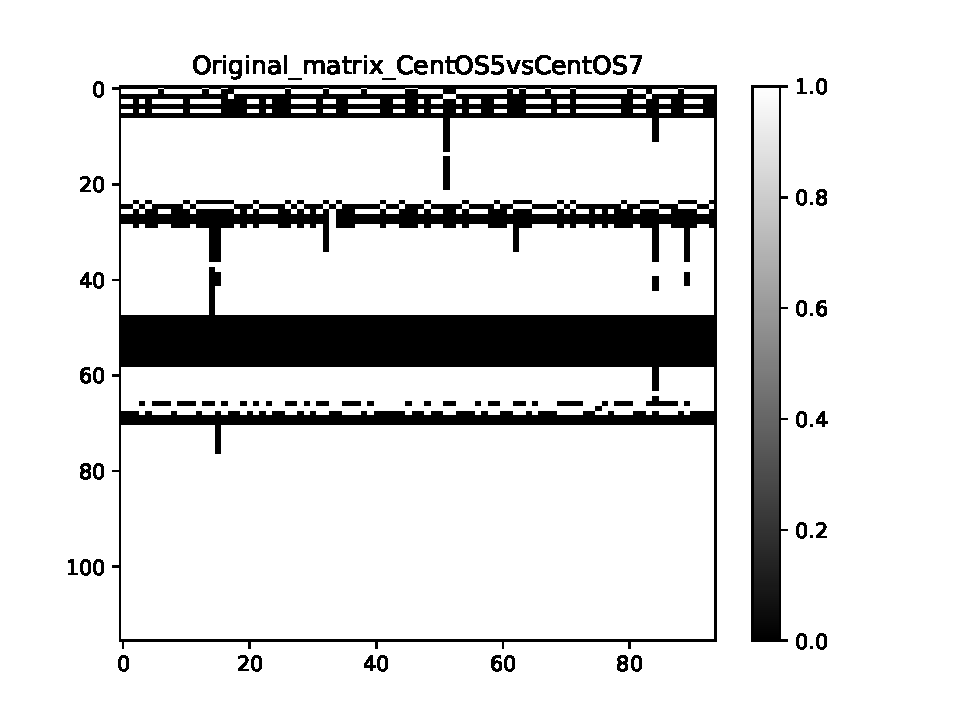
\includegraphics[width=\columnwidth]{figures/original_matrix_CentOS5vsCentOS7.pdf}
  \caption{Difference matrix, PreFreesurfer pipeline, CentOS~5 vs CentOS~7.}
  \label{fig:pre-freesurfer-5-7}
\end{figure}

% Describe your dataset: pipeline(s) used, input data, operating systems (CentOS5, 6, 7), matrix.

% 1. Prefreesurfer (what you have)
% 2. Freesurfer, with the same subjects as in Prefreesurfer.
% 3. PostFreesurfer
% 4. fmriVolume

\section{Results}

\todo{Revise intro to this section}
The experimental results have been obtained from four different approaches:
1. Applying ALS technique
2. Employing Bias as well as ALS technique
3. Using just Bias 
4. Results stemmed from ommiting the impact of predicted value of canstant files 
In all above approaches, dummy classifier which makes predictions using simple rules\cite{URL}has been used to indicate that how much predicted value would tend to be anticipate as the dominent value of the utility matrix. This classifier is considered as an accuracy evaluator since the binary utility matrix is consist of \{1,0\} which respectively represent whether a difference has been observed between the same files in two different conditions (by comapring their checksums) or not.
With the knowledge of the fact that Random Unreal method is not applicable into our case study we used its results as the comparision between the unrealistic method and realistics ones. In this regard, the aformentioned approaches are propossed and tried to lessen the gaps between the best results from random-unreal and the applied one.


\subsection{ALS without biases}

\todo{1. Use the same ordering and paragraph headings as in the method 
section. 2. Don't mix multiple ideas/results in the same paragraph. 3. 
Mention and describe the figure before discussing it.}

Results show that in all condition pairs Complete Columns method has 
almost a constant accuracy even if the training ratio increased and it 
is almost two times less than dummy classifier in more differentiated 
condition pairs (CentOS5 vs CentOS7 and CentOS6 vs CentOS7). But in the 
best case which it means in similar conditions the Complete Columns 
accuracy is as much accurate as the Dummy classifier which is $0.65$ 
percent Figure~\ref{fig:columns method} represents
the ROC curves of Complete Columns method with comparision to dummy 
classifier over the increasement of the training ratio.
\begin{figure}[h!]
        \centering
        \begin{subfigure}[b]{0.3\linewidth}
                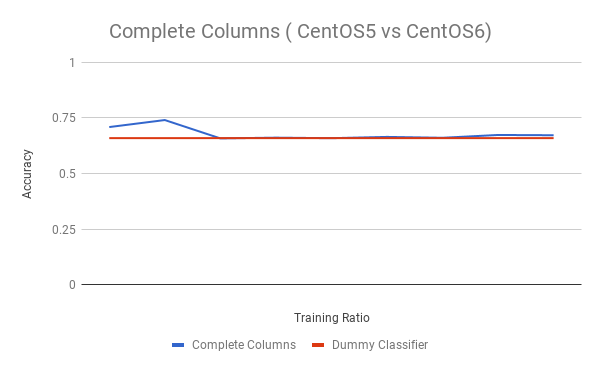
\includegraphics[width=\columnwidth]{figures/columns_5vs6}
        \end{subfigure}
        \begin{subfigure}[b]{0.3\linewidth}
                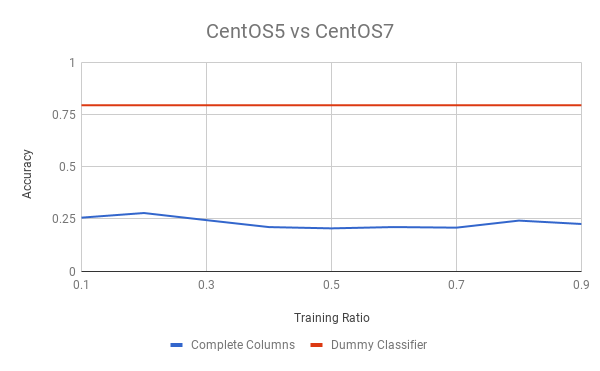
\includegraphics[width=\columnwidth]{figures/columns_5vs7}
        \end{subfigure}
        \begin{subfigure}[b]{0.3\linewidth}
                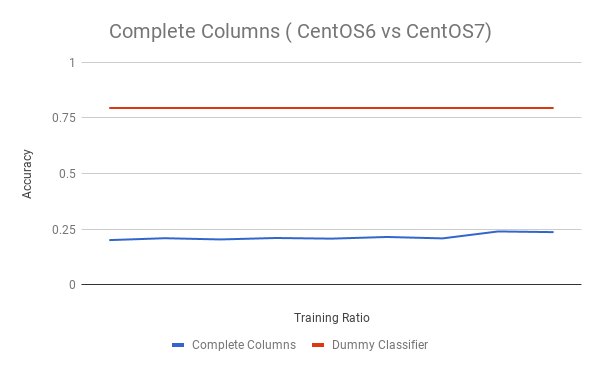
\includegraphics[width=\columnwidth]{figures/columns_6vs7}
        \end{subfigure}
        \caption{Average performance of Complete Columns methods in three different condition pairs}
        \label{fig:columns method}
\end{figure}
In general the accuracy pattern of the two Complete Rows and 
RS methods show similar decline and grow behavior over the 
training ratio axis however it can be subject to considerable 
fluctuations in differentiated condition pairs. Dispite of their 
likely irrational behaviour, they always have better accuracy 
for the training size with less than $0.3$ in comparison to other 
methods. This better performance (around 75 percent)is almost three 
times higher than other methods in condition pairs with more 
differences but just 20 percent better when the conditions are more 
similar to each other (CentOS5 vs CentOS6) with accuracy of $90\%$.
Figure~\ref{fig:RS_Rows} represents
the ROC curves of these two methods with comparision to dummy
classifier over the increasement of the training ratio.
\begin{figure}[h!]
        \centering
        \begin{subfigure}[b]{0.4\linewidth}
                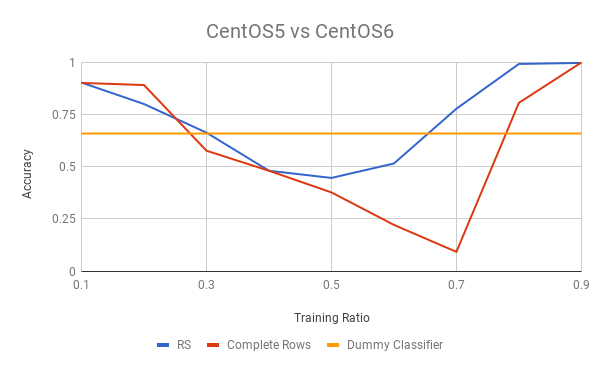
\includegraphics[width=\columnwidth]{figures/RS_Rows_5vs6}
        \end{subfigure}
        \begin{subfigure}[b]{0.4\linewidth}
                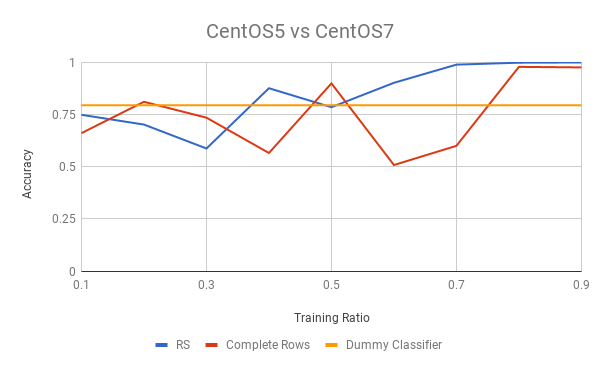
\includegraphics[width=\columnwidth]{figures/RS_Rows_5vs7}
        \end{subfigure}
        \begin{subfigure}[b]{0.4\linewidth}
                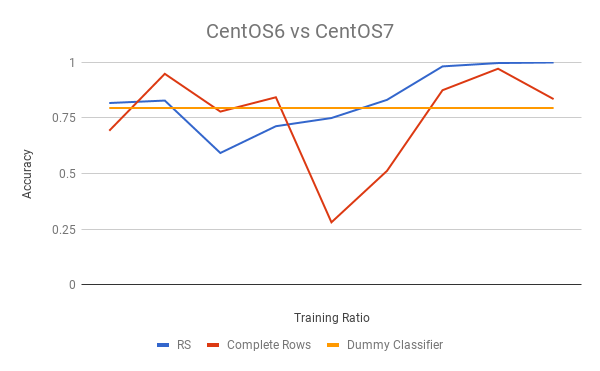
\includegraphics[width=\columnwidth]{figures/RS_Rows_6vs7}
        \end{subfigure}
        \caption{Average performance of RS and Complete Rows methods in three different condition pairs}
        \label{fig:RS_RowS}
\end{figure}

All the other random methods, RS and both RFNT approaches 
are performing a continues growth Figure~\ref{fig:simple-methods} represents
the ROC curves of all random methods with comparision to dummy
classifier over the increasement of the training ratio.. Although some considerable variation 
for both triangular approches have been observed (CentOS5 vs CentOS6) 
their constant rise leads us to the next phase of experiments which was 
adding up bias into the current ALS technique. 
The training set suffers from lacking the files which are almost generated towareds the end of pipeline.

\begin{figure}[h!]
        \centering
        \begin{subfigure}[b]{0.4\linewidth}
                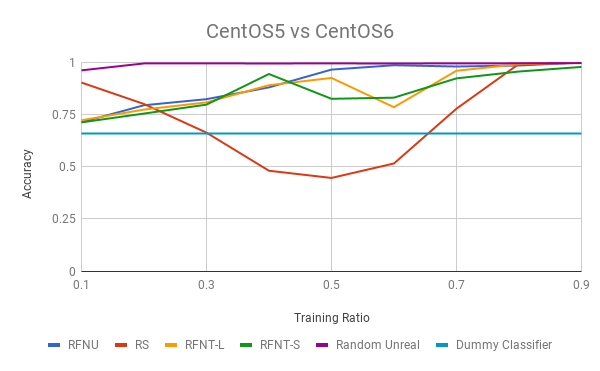
\includegraphics[width=\columnwidth]{figures/simple-methods-5vs6}
        \end{subfigure}
        \begin{subfigure}[b]{0.4\linewidth}
		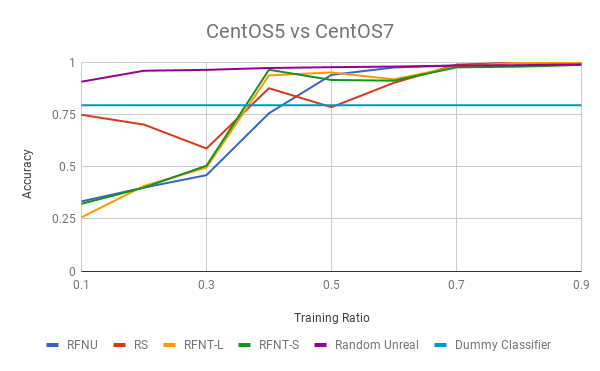
\includegraphics[width=\columnwidth]{figures/simple-methods-5vs7}
        \end{subfigure}
        \begin{subfigure}[b]{0.4\linewidth}
                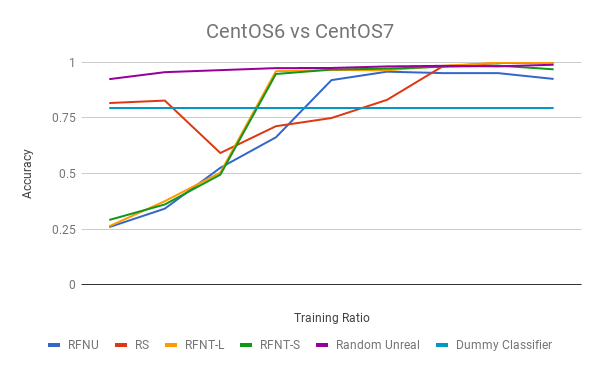
\includegraphics[width=\columnwidth]{figures/simple-methods-6vs7}
        \end{subfigure}
	\caption{Average performance of Complete Columns methods in three different condition pairs}
	\label{fig:simple-methods}
\end{figure}

% Present your results: accuracy, ROC curves, transparency matrix, factors. 

% Try with different numbers of factors. 

\section{Discussion}

% Not all subjects behave the same, which motivates the Big Data approach. 

% Which sampling method is best

% Interpreting the factors? Factors reflect the pipeline definition. 

% How can this be used in practice

% What are the limitations

\section{Conclusion}

% Summary of the results and discussion. The take-home message.

\section*{Acknowledgment}

\bibliographystyle{IEEEtran}
\bibliography{IEEEabrv,biblio.bib}


\end{document}
